\section{Optimizing init scripts and system startup}
\begin{frame}
\frametitle{Methodology}
There are multiple ways to reduce the time spent in init scripts before
starting the application:
\begin{itemize}
	\item Start the application as soon as possible after only the
              strictly necessary dependencies.
	\item Simplify shell scripts
	\item Even starting the application before \code{init}
\end{itemize}
\end{frame}

\begin{frame}
\frametitle{Measuring - bootchart}
\begin{columns}
\column{0.65\textwidth}
\begin{itemize}
	\item If you want to have a more detailed look at the userland boot sequence
              than with \code{grabserial}, you can use \code{bootchart}.
	\item \url{http://www.bootchart.org}
\end{itemize}
\column{0.35\textwidth}
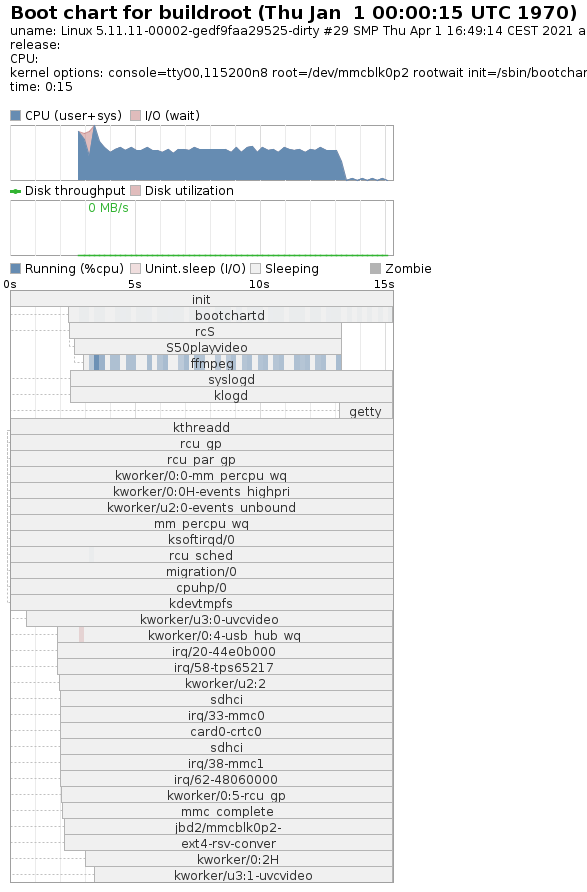
\includegraphics[height=0.85\textheight]{slides/boot-time-init-scripts/bootlog.png}
\end{columns}
\end{frame}

\begin{frame}[fragile]
\frametitle{Measuring - bootchart}
\begin{itemize}
	\item You can use \code{bootchartd} from \code{busybox}
	      (\kconfig{CONFIG_BOOTCHARTD=y})
	\item Boot your board passing \code{init=/sbin/bootchartd} on your
	      kernel command line
	\item Copy \code{/var/log/bootlog.tgz} from your target to your host
	\item The last release of Bootchart is from 2007, and is now
	      broken on \url{http://www.bootchart.org}. Download a copy
	      from \url{https://bootlin.com/pub/source/bootchart-0.9.tar.bz2}
	\item Generate the timechart:
\begin{block}{}
\begin{verbatim}
cd bootchart-<version>
java -jar bootchart.jar bootlog.tgz
\end{verbatim}
\end{block}
	\item This produces a \code{bootlog.png} image
\end{itemize}
\end{frame}

\begin{frame}[fragile]
\frametitle{Measuring - systemd}
If you are using \code{systemd} as your \code{init} program, you can use
\code{systemd-analyze}. See
\url{https://www.freedesktop.org/software/systemd/man/systemd-analyze.html}.\\
\begin{block}{}
\tiny
\begin{verbatim}
$ systemd-analyze critical-chain
multi-user.target @47.820s
└─pmie.service @35.968s +548ms
  └─pmcd.service @33.715s +2.247s
    └─network-online.target @33.712s
      └─systemd-networkd-wait-online.service @12.804s +20.905s
        └─systemd-networkd.service @11.109s +1.690s
          └─systemd-udevd.service @9.201s +1.904s
            └─systemd-tmpfiles-setup-dev.service @7.306s +1.776s
              └─kmod-static-nodes.service @6.976s +177ms
                └─systemd-journald.socket
                  └─system.slice
                    └─-.slice
\end{verbatim}
\end{block}
\end{frame}

\begin{frame}[fragile]
\frametitle{systemd-analyse plot}
\begin{columns}
\column{0.7\textwidth}
This command prints an SVG graphic detailing which system services have been started at what time,
highlighting the time they spent on initialization.
\begin{verbatim}
$ systemd-analyze plot >bootup.svg
$ inkscape bootup.svg
\end{verbatim}
\column{0.3\textwidth}
\includegraphics[width=\textwidth]{slides/boot-time-init-scripts/systemd-analyse-plot.pdf}
\end{columns}
\end{frame}


\begin{frame}
\frametitle{Init optimizations}
Goal to start your application as soon as possible after all the dependencies are started:
\begin{itemize}
	\item Depends on your \code{init} program. Here we are assuming sysV
	      \code{init} scripts.
	\item \code{init} scripts run in alphanumeric order and start with
	      a letter (K for stop ({\bf k}ill) and S for {\bf s}tart).
	\item You want to use the lowest number you can for your application.
	\item You can even replace \code{init} with your application!
\end{itemize}
How fast would we be if we could be the first started application?
\end{frame}

\begin{frame}[fragile]
\frametitle{Optimizing init scripts}
\begin{itemize}
	\item Start all your services directly from a single startup
	      script (e.g. \code{/etc/init.d/rcS}). This eliminates multiple
	      calls to \code{/bin/sh}.
	\item An easier to maintain solution allowing to keep subscripts: \code{source} them\\
              (\code{.} command) if possible. This won't spawn new shell processes.
	\item You could mount your filesystems directly in the C code
	      of your application:
\end{itemize}
\begin{block}{}
\begin{minted}[fontsize=\small]{c}
#include <stdio.h>
#include <sys/mount.h>

int main (void)
{
        int ret;
        ret = mount("sysfs", "/tmp/test", "sysfs", 0, NULL);
        if(ret < 0)
                perror("Can't mount sysfs\n");
}
\end{minted}
\end{block}
\end{frame}

\begin{frame}[fragile]
\frametitle{Reduce forking (1)}
\begin{itemize}
\item \code{fork}/\code{exec} system calls are very expensive.
      Because of this, calls to executables from shells are slow.
\item Try to use shell built-ins whenever possible. For example in
      BusyBox, you can use \code{echo}, \code{test}, \code{printf}
      and others as shell built-ins.
\item Pipes and back-quotes are also implemented by
      \code{fork}/\code{exec}.  You can reduce their usage in
      scripts. Example:
      \begin{block}{}
      \begin{verbatim}
cat /proc/cpuinfo | grep model
      \end{verbatim}
      \end{block}
Replace it with:
      \begin{block}{}
      \begin{verbatim}
grep model /proc/cpuinfo
      \end{verbatim}
      \end{block}
\end{itemize}
See \url{https://elinux.org/Optimize_RC_Scripts}
\end{frame}

\begin{frame}[fragile]
\frametitle{Reduce forking (2)}
Replaced:
\begin{block}{}
\begin{verbatim}
if [ $(expr match "$(cat /proc/cmdline)" '.* debug.*')\
       -ne 0 -o -f /root/debug ]; then
DEBUG=1
\end{verbatim}
\end{block}
By a much cheaper command running only one process:
\begin{block}{}
\begin{verbatim}
res=`grep " debug" /proc/cmdline`
if [ "$res" -o -f /root/debug ]; then
DEBUG=1
\end{verbatim}
\end{block}
This only optimization allowed to save 87 ms on an ARM AT91SAM9263
system (200 MHz)!
\end{frame}


\begin{frame}
\frametitle{Reduce size (1)}
\begin{itemize}
	\item Strip your executables and libraries, removing ELF sections
		only needed for development and debugging. The \code{strip}
		command is provided by your cross-compiling toolchain.
		That's done by default in Buildroot.
	\item \code{superstrip}:
		\url{https://muppetlabs.com/~breadbox/software/elfkickers.html}.
		Goes beyond \code{strip} and can strip out a few more bits
		that are not used by Linux to start an executable.
		Buildroot stopped supporting it because it can break
	        executables. Try it only if saving a few bytes is
		critical.
\end{itemize}
\end{frame}

\begin{frame}
\frametitle{Reduce size (2)}
You may try \code{mklibs}, available at \url{https://packages.debian.org/sid/mklibs}.
\begin{itemize}
	\item \code{mklibs} produces cut-down shared libraries that contain
	only the routines required by a particular set of executables.
	Really useful with big libraries like OpenGL and QT. It even
	works without having the source code.
	\item Available in Yocto, but not in Buildroot (2021.02 status).
        \item Limitation: \code{mklibs} could remove \code{dlopen}ed libraries
        (loaded "manually" by applications) because it doesn't see them.
\end{itemize}
\end{frame}

\begin{frame}
\frametitle{Quick splashscreen display (1)}
Often the first sign of life that you are showing!
\begin{itemize}
\item A good solution seems to be BusyBox \code{fbsplash}:\\
      See \projfile{busybox}{miscutils/fbsplash.c} in BusyBox sources.
\item Alternative: \code{fbv}\\
      \url{http://s-tech.elsat.net.pl/fbv/}
\item However, \code{fbv} is slow:\\
      878 ms on an Microchip AT91SAM9263 system!
\end{itemize}
\end{frame}

\begin{frame}[fragile]
\frametitle{Quick splashscreen display (2)}
\begin{itemize}
\item To do it faster, you can dump the framebuffer contents:\\
      \begin{verbatim}
fbv -d 1 /root/logo.bmp
cp /dev/fb0 /root/logo.fb
lzop -9 /root/logo.fb
      \end{verbatim}
\item And then copy it back as early as possible in an initramfs:
      \begin{verbatim}
lzopcat /root/logo.fb.lzo > /dev/fb0
      \end{verbatim}
\end{itemize}
Results on an Microchip AT91SAM9263 system: \\
\begin{tabular}{| l || c | c | c | }
\hline
& \code{fbv} & plain copy (\code{dd}) & \code{lzopcat} \\
\hline
Time & 878 ms & 54 ms & 52.5 ms\\
\hline
\end{tabular}
\vfill
\footnotesize
\url{https://bootlin.com/blog/super-fast-linux-splashscreen/} \\
Note: {\em LZO} compression is the fastest in terms of
decompression, and is supported by BusyBox.
\end{frame}

\begin{frame}
\frametitle{Animated splashscreen}
Still slow to read and write entire screens. Just draw useful pixels
and even create an animation!
\begin{itemize}
\item Create a simple C program that just animates pixels and simple
      geometric shapes on the framebuffer!
\item Example: {\small \url{https://bootlin.com/pub/code/fb/anim.c}}
      (Public Domain license).\\
      On a 400 MHz ARM9 system: starts drawing in 10 ms \\
      Size: 24 KB, compiled statically.
\end{itemize}
\end{frame}


\setuplabframe
{Reducing time in init-scripts}
{
\begin{itemize}
\item Regenerate the root filesystem with Buildroot
\item Use bootchartd to measure boot time
\end{itemize}
}
